\section{Discussion of Results}\label{sec:result}

\subsubsection{Evaluation Against Other Approaches}

\begin{figure}
    \centering
    % First figure
    \begin{minipage}[t]{0.40\linewidth}
        \centering
        \includegraphics[width=\linewidth]{analysis/artefact/variation_approach/reduction_query_execution_time_raw}
    \end{minipage}
    \hspace{0.05\textwidth}
    % Second figure
    \begin{minipage}[t]{0.40\linewidth}
        \centering
        \includegraphics[width=\linewidth]{analysis/artefact/variation_approach/reduction_query_execution_time}
    \end{minipage}

    % General caption
    \caption{
        On the left a plot of the query execution time and on the right the figure compares the type index with the LDP approach against other approaches.
        The shape index approach is faster or similar to the other approach except for S4.
        }
    \label{fig:compApproach}
\end{figure}

%\input{analysis/artefact/statistical_significance/comparaisonStateOfTheArt}


Figure~\ref{fig:compApproach} shows that the shape index approach for all query templates except S4 performs better or comparably to the state-of-the-art Solid Pod network traversal algorithm.
An analysis of statistical significance is provided in the supplementary material~\hyperref[sf:complementaryMaterial]{\footnotemark[\getrefnumber{sf:complementaryMaterial}]}.
Queries can require as little as 13\% or 7.7 times less (S1) of the execution time of the type index and LDP traversal algorithm.
Queries that perform best are those where the number of HTTP requests decreased the most.
%Table~\ref{tab:statSignificanceStateOfTheArt} presents an analysis of the statistical significance of the query template and its relation to the ratio of HTTP requests performed.
Queries from templates D6 and D7 show no reduction because they require nearly every document in the dataset to be processed by the engine, making our approach ineffective in these cases.
We notice that queries from template S4 with the shape index performed worse in every instance, with an increase in query execution time of up to 2.80 times.
\input{analysis/artefact/ratio_useful_resources/table_ratio_useful_ressources}
This is further illustrated in Table~\ref{tab:ratioUsefulResources}, which shows that for these queries, the type index and LDP traversal algorithm achieves a ratio of useful resources dereferenced of 100\% or 50\%, compared to only 6\% with the shape index approach.
The poor performance is due to the fact that other approaches rely solely on the reachability \texttt{Cmatch}~\cite{hartig2016walking} to achieve completeness, without leveraging the structural properties of the datasets.
In contrast, the shape index approach always enforces the use of these properties, resulting in additional HTTP requests and increased processing time.
It has to be highlighted that our formalization assumes that structural assumptions are always used and that the shape index, if present, will be part of the traversal, see section~\ref{sec:sourceSelection}.
However, those queries were already fast, with the type index and LDP traversal algorithm approach being executed in approximately 0.30\% of the maximum execution time allowed.
Nonetheless, these results still highlight a category of queries and networks for which our approach is not well-suited.
Those results mostly validate \textbf{H1} however the shape index approach can drastically increase the execution time when the structural properties are not used.

\subsubsection{Query-Shape Containment Evaluation}
The empirical evaluation of the query-shape containment algorithm shows that its execution time with the more detailed shapes from our experiment is negligible, with a maximum execution time of 4.655 ms (0.0039\% of the timeout).
The result tables are available in the supplementary material~\hyperref[sf:complementaryMaterial]{\footnotemark[\getrefnumber{sf:complementaryMaterial}]}.
This outcome is expected, as the algorithm has polynomial time complexity, and the shapes and queries in the experiments are small and not deeply nested.
This result validated \textbf{H2}.

\iffalse
\begin{figure}[htbp]
    \centering
    % First figure
    \begin{minipage}[t]{0.40\linewidth}
        \centering
        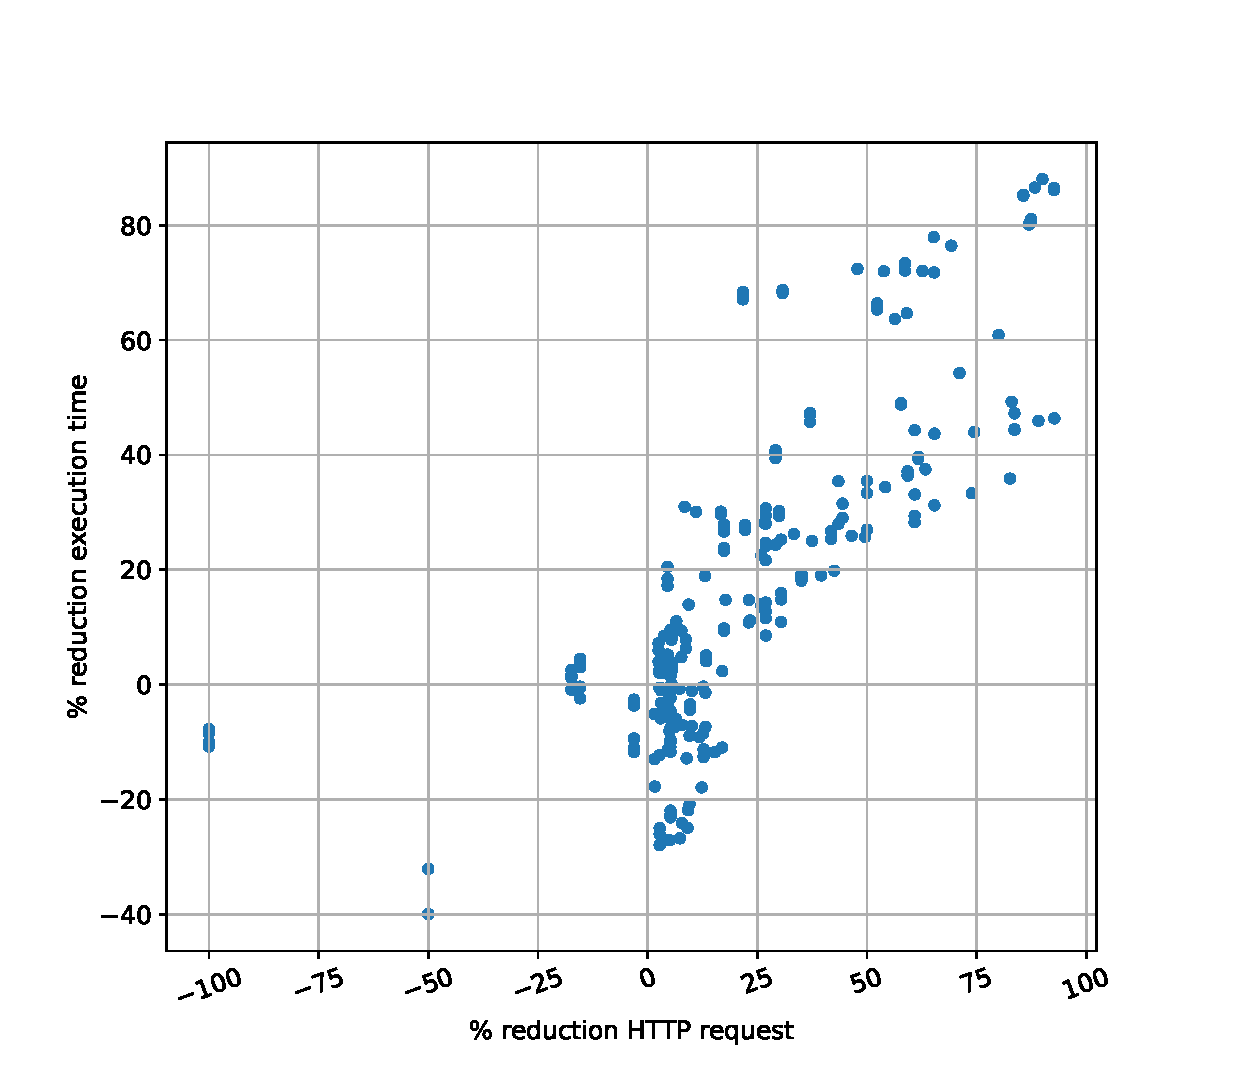
\includegraphics[width=\linewidth]{analysis/artefact/http_req_exec_time_relation/http_req_exec_time_cor_better}
        \label{fig:http_req_exec_time_cor_better}
    \end{minipage}
    \hspace{0.05\textwidth}
    % Second figure
    \begin{minipage}[t]{0.40\linewidth}
        \centering
        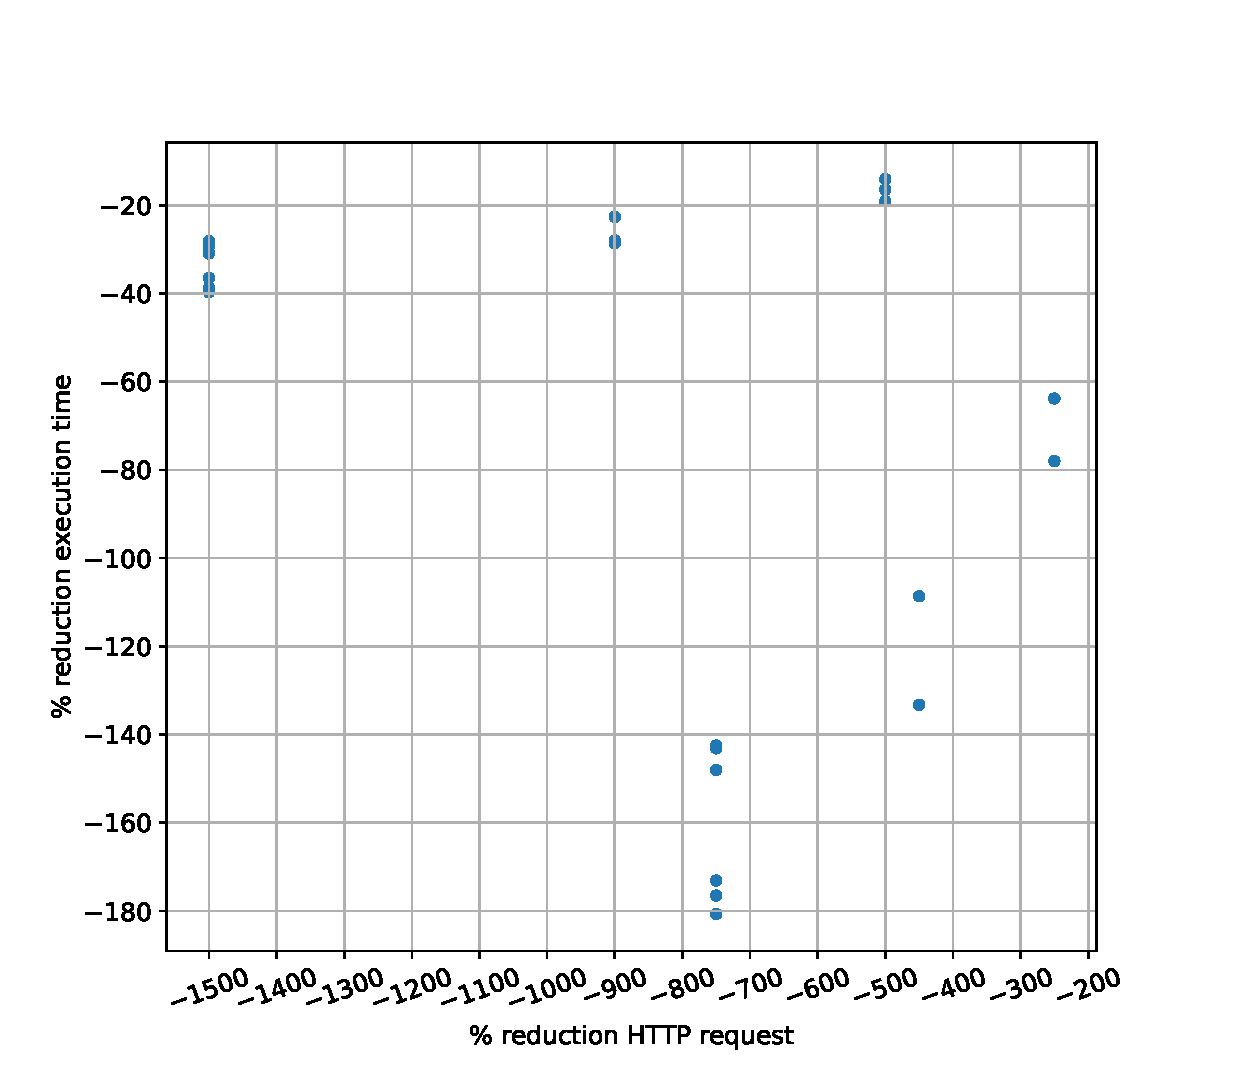
\includegraphics[width=\linewidth]{analysis/artefact/http_req_exec_time_relation/http_req_exec_time_cor_worse}
        \label{fig:http_req_exec_time_cor_worse}
    \end{minipage}

    % General caption
    \caption{
        The data show two regimes in the relation between the number of HTTP requests and the execution time, 
        we see a more linear correlation on the left figure than on the right figure.
        }
    \label{fig:http_req_exec_time_cor}
\end{figure}

\subsubsection{Relationship Between HTTP Request and Query Execution Time}

To determine the relationship between the reduction of HTTP requests and the query execution time, we evaluated their ratio using 
the data of our experiments with the Solid Pod network optimal traversal algorithm results as the baseline.
Figure~\ref{fig:http_req_exec_time_cor} present our analysis.
The relationship between HTTP request and query execution time can be divided into two regimes.
In the first regime (left figure), where the shape index approach reduces the number of HTTP requests, we notice a positive linear correlation with a
Pearson correlation coefficient (PCC) of 0.84 and a high statistical significance given $< 0.01$.
We can notice that toward the end, the curve appears to exhibit more exponential behavior.
Evaluating an $R^2$ score with an exponential best fit curve we get a score of 0.72 and 0.71 for a linear curve.
Below a ratio of approximately 0.83 of HTTP requests, the shape index approach did not guarantee a reduction in query execution time.
With this observation, the exponential behavior might be explained by the approach's overhead. 
It is possible that with a small reduction of HTTP requests, the state retention required for the pruning reachability criteria could offset the gain in the reduction of HTTP requests.
In the second regime (right figure), the shape index increases the number of HTTP requests.
We notice a weaker positive linear correlation with a PCC of 0.44 and a high statistical significance though the significance is lower than in the first regime.
The overall correlation between reducing HTTP requests and query execution time is positively linear, with a PCC of 0.56 and a high statistical significance.
The overall correlation is more linear than exponential with $R^2$ scores respectively of 0.31 and 0.24, however due to the low score it is difficult to determine the nature of the distribution.
Explaining the two regimes' behavior exhibited by the data is challenging.
A possible explanation can be the lack of samples when the shape index approach performs poorly.
However, we can also notice that the relationship between the two variables in the first regime is closer to one-on-one (slope of approximately 0.91) than in the second regime (slope of approximately 0.08), where the ratio of HTTP requests has less of an impact.
Futhermore, the number of HTTP requests increased by 16 times compared to the baseline, which initially required only 1 or 2 requests (see Table ~\ref{tab:ratioUsefulResources}). 
However, despite this increase, the engine ultimately handled a modest number of links to dereference.
This indicates that the actual impact might not be as significant as the figure suggests, particularly considering that HTTP requests are done concurrently.
Those results validate \textbf{H2} when there is a decrease in HTTP requests, however, with an increase, the results are more uncertain.
%\rt{I think this paragraph can be shorted quite a bit if you run into space issues.}
%This observation can lead us to question how complex the queries are in that regime; queries where the shape index increases vastly in the number of HTTP requests are the queries from the S4 template. 
%However, those queries were already answered quickly and consisted of only four triple patterns and a union statement (with the alternative property path). 
%Thus, it is possible that the number of HTTP requests has less of an impact because it is easier for the engine to perform the join operation upon reception of the data than when processing more complex queries.
%Additionally, those queries where already answer with 1 or 2 HTTP request with the baseline thus increase by 16 time of the number of HTTP request still leave the engine with a modest number of links to dereference.

% Analysis by query template? But we lack the space. In the appendix too...
% We can also with that explain some big gap in the plot.
\fi


\subsubsection{Evaluation of the Resilience of the approach}

The final part of the results analysis focuses on the resilience of the shape index approach.
In this analysis, we examine the impact of reducing the shape index information in the network and compare the results with a network in which all pods are exposed to detailed, complete shape indexes.
Figure~\ref{fig:adaptShapeIndex} presents three plots that illustrate the results of our evaluation of the approach's resilience.
The plot on the left shows the variation in the availability of shape indexes across the network. 
As expected, we observe that queries that performed better in Figure~\ref{fig:compApproach} tend to perform worse with reduced shape index information, while queries that performed poorly improve. 
Queries that were unaffected by the shape index changes remain unaffected.


\begin{figure}
    \centering
    \includegraphics[width=1\linewidth]{analysis/artefact/variation_shape_index_all/plot}
    \caption{
    Shape index approaches tend to perform less effectively with limited network information and comparatively better where the baseline shape index underperforms.
    However, the utility of shape index information can vary depending on the specific queries and network characteristics.
    }
    \label{fig:adaptShapeIndex}
\end{figure}

The plot in the middle shows the variation in the percentage of shape index entries using closed shapes.
The results here are more nuanced.
While there is a general trend for query evaluations with a lower percentage of closed shapes to behave similarly to the plot on the left, we also observe both performance gains for some query template and a drastic performance loss for the queries of S1 when 80\% of the shape entries are closed.
The performance gain occurs because not every entry needs to be closed to prune the query irrelevant documents.
Entries mapped to an open shape are always considered relevant because the shape translate to a query fetching the whole KG.
If the containment resolution leads to the same conclusion then given a closed entry, the execution will be more expensive because 
when shape are nested, the nested shapes need to be dereference to solve the query-shape containment algorithm.
For the queries of S1, with 80\% of closed shape entries, the performance lost was due to random chance, as the discriminatory entries were provided with open shapes in multiple instances when looking at the raw data.

The right plot shows the variation in the level of detail of the shapes by reducing their detail.
Since the shapes are closed in this experiment the level of detail was varied by changing the constraint of the object terms of the shape as describe in Section~\ref{sec:experiment}.
Most queries tend to perform similarly or better, with the exception of those of S1.
Upon analyzing the output of our query containment algorithm, we observe that the additional information to the shape provided in our base approach does not affect the algorithm’s results.
However, the engine needs to dereference more shapes, which can increase the execution time.
Queries of template S1 is the only one where the added information can discriminate multiple parts of the datasets' domain, indicating the intuitive results that, in some situations, adding more information can be beneficial.
This sensitivity of the quantity of the information in the index also helps explain the results for S1 queries in the middle plot. 
In that case, the query engine still had to dereference sources from each dataset, and the information available was likely insufficient to significantly discriminate between sources.

Those results shows that \textbf{H3} is mainly invalid; reducing information is rarely detrimental for query execution, except in cases where added information is critical to determine the query relevance of sources.
Thus, this outcome is query-dependent.
\textbf{H4} and \textbf{H5} are valid but show that the completeness of shape indexes has less impact on performance than the absence of indexes.
Incomplete shape indexes can increase performance surprisingly if incomplete entries are not necessary to discriminate irrelevant sources. 
Like with \textbf{H3}, these findings are query-dependent and also network-dependent.

